\chapter{Fase II: resultados con las condiciones de 2025}\label{cap:resultados}

\section{La trayectoria sin nuevas decisiones}

En el diseño base (solo proyectos comprometidos), la Línea 1, la troncal de la avenida 68 y el
Regiotram de Occidente reducen el tiempo medio de viaje entre 2027 y 2030, pero el crecimiento de la
demanda, sobre todo regional, lo eleva después: en 2050 el tiempo medio esperado es de
\TiempoBaseFin{} minutos y la velocidad vial en hora pico de \VelBaseFin{} km/h, con un percentil 95
del tiempo medio de \TiempoBasePNovFin{} minutos (\cref{fig:trayectorias}). La asimetría de las bandas
es la huella de la no linealidad de la congestión: los escenarios de alta demanda empeoran el sistema
mucho más de lo que lo alivian los de baja demanda, y por eso el costo esperado es mayor que el costo en
la demanda esperada.

\begin{figure}[ht]
\centering
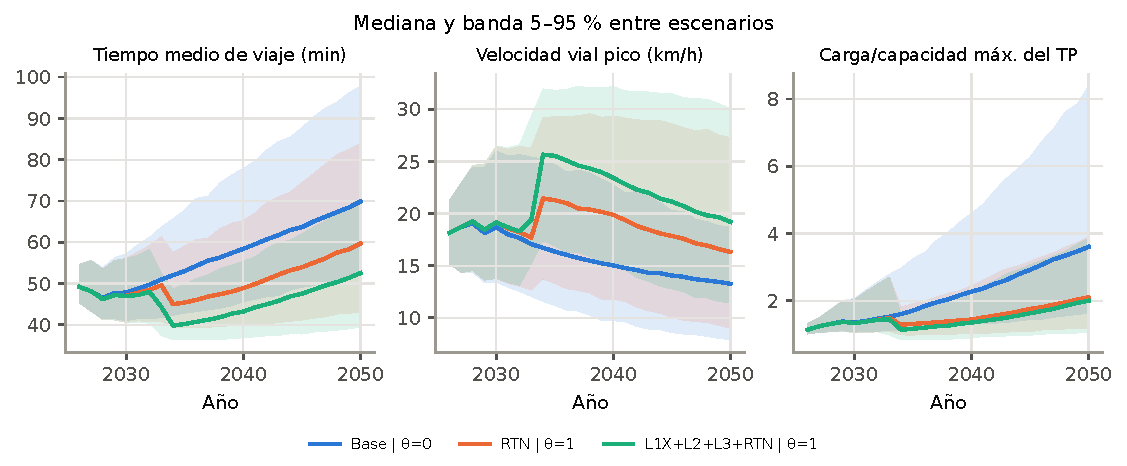
\includegraphics[width=\textwidth]{figuras/fig_trayectorias.pdf}
\caption{Tiempo medio de viaje, velocidad vial y carga máxima del TP: mediana y banda 5--95\,\% para
el diseño base, el óptimo y el diseño con todos los proyectos.}\label{fig:trayectorias}
\end{figure}

\section{Comparación de diseños}

La \cref{tab:disenos} presenta los doce diseños de menor costo esperado y algunos de referencia, y la
\cref{fig:frontera} los \NDisenos{} diseños en el plano media--CVaR. Cuatro resultados destacan.

\begin{table}[ht]
\centering\small
\caption{Diseños ordenados por costo social esperado (VP 2026, billones de pesos). BN: beneficio neto
frente al diseño base; CAPEX esperado con sobrecostos; $\bar t_{2050}$: tiempo medio de viaje esperado
en 2050.}\label{tab:disenos}
\resizebox{\textwidth}{!}{\begin{tabular}{p{4.1cm}rrrrrrc}
\toprule
Diseño & E[VP] & CVaR$_{95}$ & E[BN] & P(BN$>$0) & CAPEX & $\bar t_{2050}$ & Pareto \\
 & \multicolumn{3}{c}{billones COP} & & billones & min & \\
\midrule
RTN \textbar{} $\theta$=1 & 292,3 & 432,7 & 16,6 & 98\,\% & 6,2 & 60,8 & \checkmark \\
L1X+\allowbreak{}RTN \textbar{} $\theta$=1 & 294,2 & 432,1 & 14,6 & 96\,\% & 11,1 & 60,2 & \checkmark \\
RTN \textbar{} $\theta$=0{,}5 & 296,2 & 443,3 & 12,6 & 98\,\% & 6,2 & 62,8 &  \\
L1X+\allowbreak{}RTN \textbar{} $\theta$=0{,}5 & 298,0 & 442,4 & 10,8 & 94\,\% & 11,1 & 62,1 &  \\
Base \textbar{} $\theta$=1 & 299,7 & 445,3 & 9,1 & 100\,\% & 0,0 & 67,4 &  \\
L1X \textbar{} $\theta$=1 & 300,5 & 441,6 & 8,3 & 93\,\% & 4,9 & 66,1 &  \\
RTN \textbar{} $\theta$=0 & 300,8 & 455,3 & 8,0 & 94\,\% & 6,2 & 65,2 &  \\
L1X+\allowbreak{}RTN \textbar{} $\theta$=0 & 302,5 & 453,8 & 6,3 & 88\,\% & 11,1 & 64,4 &  \\
Base \textbar{} $\theta$=0{,}5 & 303,9 & 456,4 & 4,9 & 100\,\% & 0,0 & 69,4 &  \\
L1X \textbar{} $\theta$=0{,}5 & 304,5 & 452,0 & 4,3 & 84\,\% & 4,9 & 68,0 &  \\
L2+\allowbreak{}RTN \textbar{} $\theta$=1 & 306,6 & 440,9 & 2,2 & 52\,\% & 34,7 & 59,3 &  \\
L1X+\allowbreak{}L2+\allowbreak{}RTN \textbar{} $\theta$=1 & 308,5 & 440,2 & 0,3 & 45\,\% & 39,6 & 58,7 &  \\
Base \textbar{} $\theta$=0 & 308,8 & 468,8 & 0,0 & 0\,\% & 0,0 & 71,7 &  \\
L2 \textbar{} $\theta$=0 & 321,4 & 472,6 & -12,5 & 3\,\% & 28,4 & 69,4 &  \\
L3 \textbar{} $\theta$=0 & 323,7 & 462,4 & -14,9 & 11\,\% & 45,8 & 64,0 &  \\
L1X+\allowbreak{}L2+\allowbreak{}L3+\allowbreak{}RTN \textbar{} $\theta$=1 & 329,1 & 445,8 & -20,3 & 14\,\% & 85,4 & 53,0 &  \\
\bottomrule
\end{tabular}
}
\end{table}

\begin{figure}[ht]
\centering
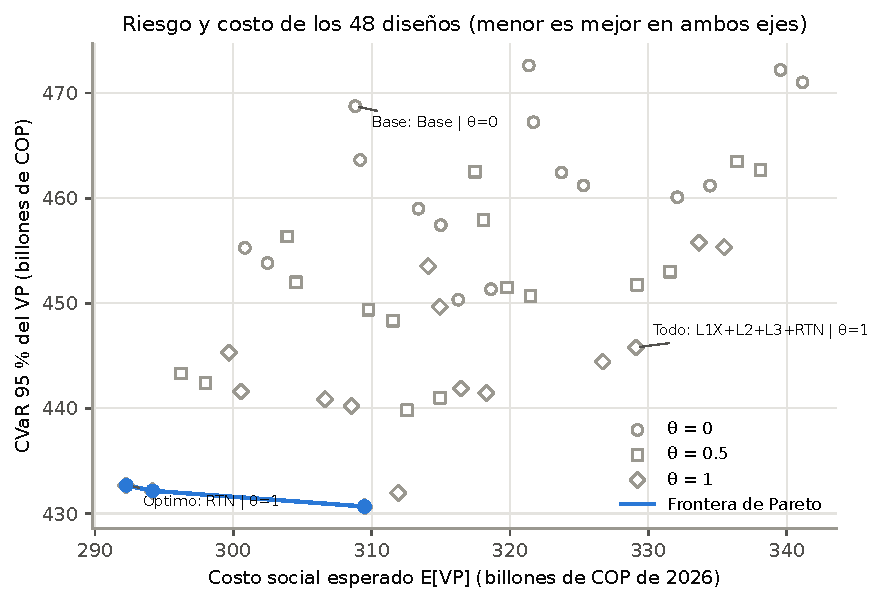
\includegraphics[width=.92\textwidth]{figuras/fig_frontera.pdf}
\caption{Costo esperado y CVaR al 95\,\% de los \NDisenos{} diseños.}\label{fig:frontera}
\end{figure}

\paragraph{1. La política de suelo es el componente más valioso por peso invertido.} Por sí sola, la
política de proximidad y policentrismo plena ($\theta=1$) tiene un beneficio neto esperado de
\BNThetaUno{} billones y es positiva en todos los escenarios. Su ventaja es que actúa sobre la demanda
en todos los corredores a la vez, mientras que cada proyecto férreo alivia uno o dos.

\paragraph{2. El Regiotram del Norte es el único proyecto en decisión con beneficio esperado positivo
y robusto.} Solo, su beneficio neto esperado es \BNRTN{} billones (positivo en el \PBNRTN{} de los
escenarios). El corredor de la Sabana Norte combina el crecimiento más alto de la demanda con la menor
capacidad de TP de la red, de modo que su saturación es probable y el proyecto es barato frente a una
línea de metro.

\paragraph{3. El diseño óptimo es \OptimoNeutral.} Con la política de suelo plena y el Regiotram del
Norte, el costo esperado baja de \VPBase{} a \VPOptimo{} billones, el CVaR de \CVaRBase{} a
\CVaROptimo, y el beneficio neto esperado es \BNOptimo{} billones (error estándar \BNOptimoEE),
positivo en el \PBNOptimo{} de los escenarios. Es óptimo para todo peso del CVaR $w<\WCambio$; desde ese
valor, el diseño que minimiza \eqref{eq:problema} agrega la extensión de la Línea 1, cuyo CVaR es
prácticamente igual, y solo con $w=1$ (un planificador que mira exclusivamente la cola) el elegido es
\DisenoWAlto, que tiene el menor CVaR de todos. La frontera de Pareto está formada por esos tres
diseños.

\paragraph{4. Las líneas de metro adicionales reducen el riesgo pero no compensan su costo a la tasa de
descuento oficial.} La Línea 2 sola tiene un beneficio neto esperado de \BNLdos{} billones
(\PBNLdos{} de probabilidad de ser positivo) y la Línea 3 de \BNLtres{} (\PBNLtres). Ambas reducen
la dispersión del costo: la desviación estándar del VP pasa de \DesvBase{} billones en la base a
\DesvLtres{} con la Línea 3 y a \DesvTodo{} con todos los proyectos, porque la capacidad adicional es más
valiosa justo en los escenarios de alta demanda. El diseño con todos los proyectos logra el menor tiempo
de viaje en 2050 (\TiempoTodoFin{} minutos, frente a \TiempoOptFin{} del óptimo), pero su beneficio
neto esperado es \BNTodo{} billones.

La \cref{fig:distribucion} muestra la distribución completa del beneficio neto y la
\cref{fig:componentes} su descomposición: en los diseños con metro, los ahorros de tiempo son grandes,
pero la inversión con sobrecostos los supera.

\begin{figure}[ht]
\centering
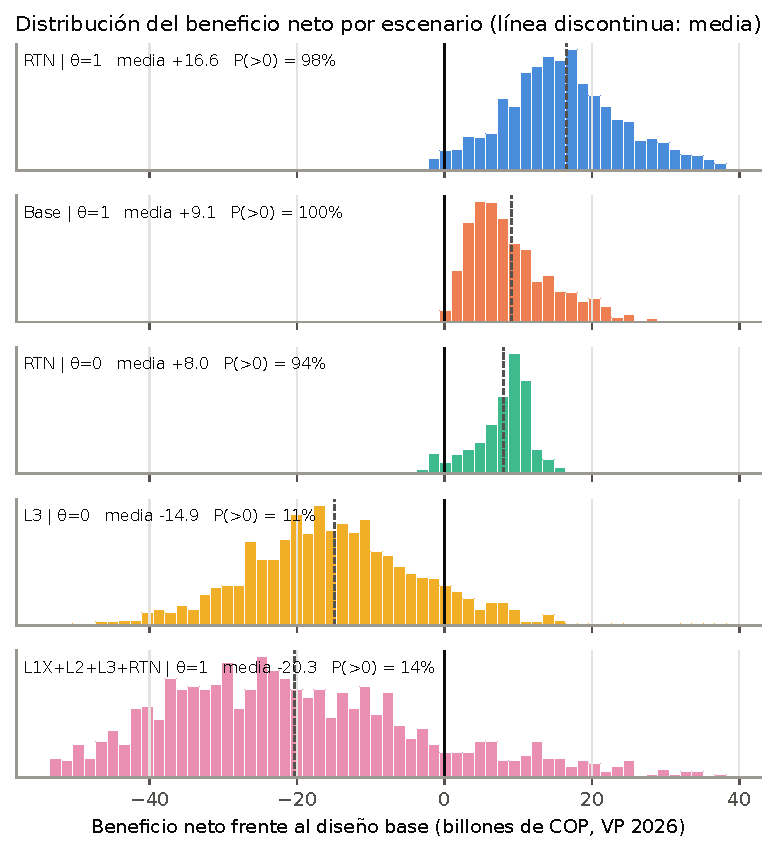
\includegraphics[width=.92\textwidth]{figuras/fig_distribucion.pdf}
\caption{Distribución del beneficio neto frente al diseño base en los \NEscenarios{} escenarios.}\label{fig:distribucion}
\end{figure}

\begin{figure}[ht]
\centering
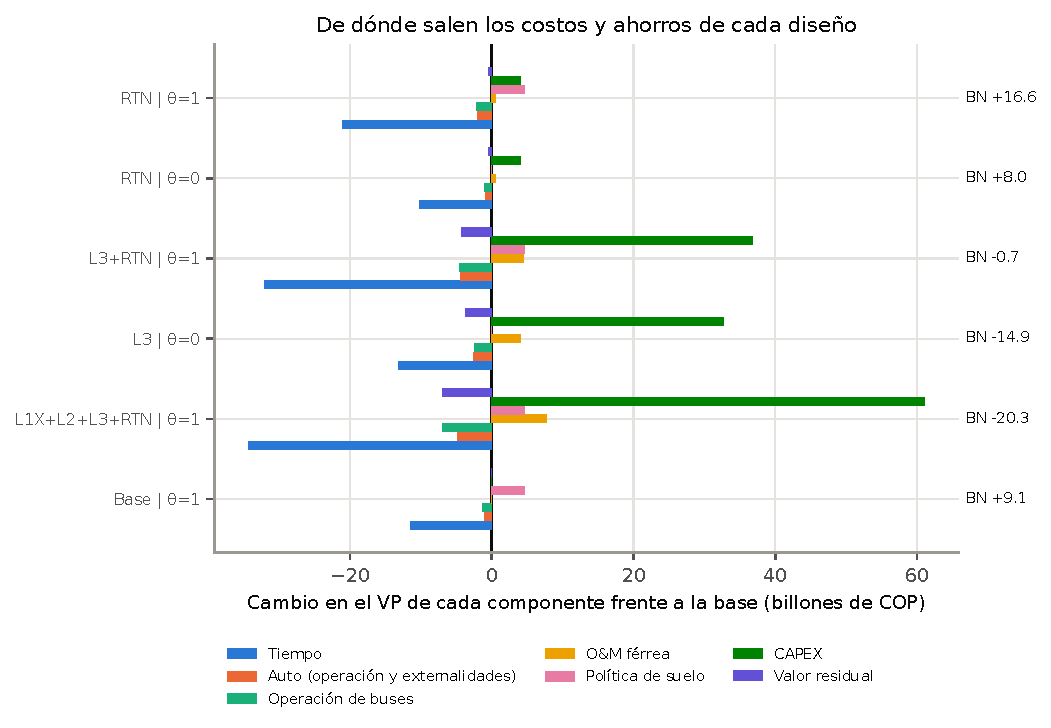
\includegraphics[width=.92\textwidth]{figuras/fig_componentes.pdf}
\caption{Cambio en el valor presente de cada componente del costo frente al diseño base.}\label{fig:componentes}
\end{figure}

\section{Sensibilidad}

La \cref{fig:tornado} varía un parámetro a la vez y recalcula el beneficio neto esperado del diseño
óptimo con \NSens{} escenarios (caso central: \BNCentralSens{} billones). Los factores más influyentes
son el valor del tiempo, la tasa de descuento y el número de horas pico equivalentes por año, seguidos
de la fracción de viajes que la política de suelo convierte a modos no motorizados. En ningún caso el
beneficio neto cambia de signo. La volatilidad del factor común casi no altera el beneficio esperado del
óptimo, aunque sí altera el riesgo de los diseños con metro.

\begin{figure}[ht]
\centering
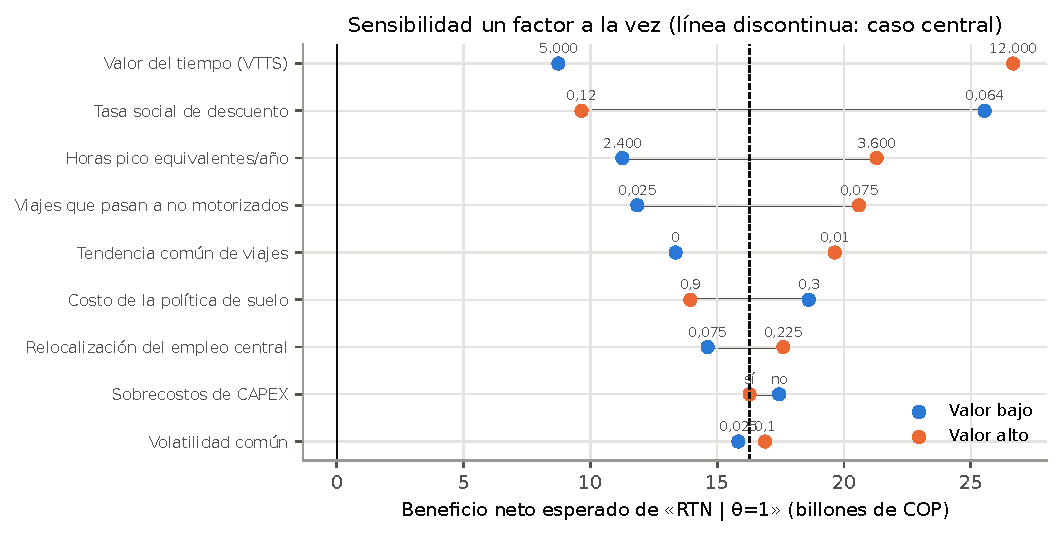
\includegraphics[width=.92\textwidth]{figuras/fig_tornado.pdf}
\caption{Sensibilidad del beneficio neto esperado del diseño óptimo a un parámetro a la vez.}\label{fig:tornado}
\end{figure}

\subsection{La tasa social de descuento}

La tasa de descuento merece atención aparte, porque las líneas de metro concentran su costo al
principio y sus beneficios después (\cref{tab:descuento}, \cref{fig:descuento}). El diseño óptimo
domina a todas las tasas estudiadas, pero el orden de los demás cambia: con 6,4\,\% el diseño
\texttt{L3+RTN | θ=1} ya tiene beneficio neto esperado positivo, y con 3,5\,\% también lo tiene el
diseño con todos los proyectos. La Línea 2 sola, en cambio, no es rentable en este modelo a ninguna de
las tasas consideradas, y la Línea 3 sola solo pasa a ser positiva con 3,5\,\% (\LtresDescTres{}
billones).
La elección de la tasa es, en buena medida, una elección sobre cuánto pesa el bienestar de las
generaciones futuras, y no un parámetro técnico.

\begin{table}[ht]
\centering\small
\caption{Beneficio neto esperado (billones de pesos) según la tasa social de descuento.}\label{tab:descuento}
\begin{tabular}{p{4.6cm}rrrr}
\toprule
Diseño & 3,5\,\% & 6,4\,\% & 9,0\,\% & 12,0\,\% \\
\midrule
Base \textbar{} $\theta$=1 & 22,6 & 13,9 & 9,1 & 5,7 \\
L1X+\allowbreak{}L2+\allowbreak{}L3+\allowbreak{}RTN \textbar{} $\theta$=1 & 25,2 & -5,7 & -20,3 & -28,8 \\
L2 \textbar{} $\theta$=0 & -5,4 & -10,5 & -12,5 & -13,3 \\
L3 \textbar{} $\theta$=0 & 3,4 & -9,2 & -14,9 & -17,9 \\
L3+\allowbreak{}RTN \textbar{} $\theta$=1 & 41,5 & 13,4 & -0,7 & -9,6 \\
RTN \textbar{} $\theta$=0 & 21,9 & 12,9 & 8,0 & 4,5 \\
RTN \textbar{} $\theta$=1 & 43,2 & 26,0 & 16,6 & 9,8 \\
\bottomrule
\end{tabular}

\end{table}

\begin{figure}[ht]
\centering
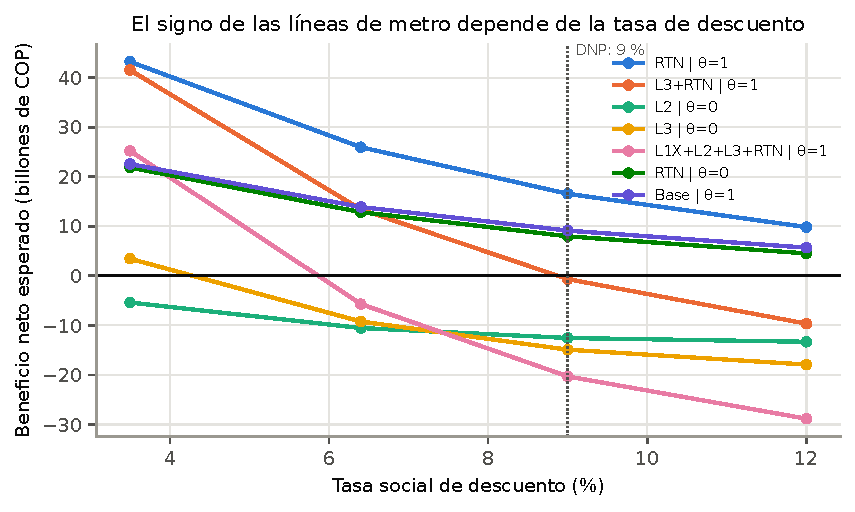
\includegraphics[width=.86\textwidth]{figuras/fig_descuento.pdf}
\caption{Beneficio neto esperado y tasa social de descuento.}\label{fig:descuento}
\end{figure}

\section{Choques sistémicos}

Para representar eventos como la pandemia se repitió la evaluación de siete diseños con saltos de
Merton en el factor común: intensidad de 0,04 por año (un choque cada 25 años en promedio), tamaño
logarítmico medio de $-0{,}35$ y desviación de 0,10, con compensación de la deriva para que la demanda
esperada no cambie (\cref{tab:saltos}). Aunque la demanda media es la misma, el costo esperado sube,
porque el costo es convexo en la demanda y los saltos ensanchan la distribución, y el CVaR aumenta
mucho más: el del diseño base pasa de \CVaRMBGBase{} a \CVaRSaltosBase{} billones. Con saltos, el diseño
\texttt{L3+RTN | θ=1} pasa a tener el menor CVaR de los evaluados, de modo que para un planificador muy
averso al riesgo (peso del CVaR superior a \WSaltos{} entre esos siete diseños) la Línea 3 entra en el
diseño óptimo. La Línea 3 actúa como un seguro contra escenarios extremos: su valor depende de cuánto
peso se dé a esos escenarios.

\begin{table}[ht]
\centering\small
\caption{Costo esperado y CVaR (billones de pesos) con MBG y con MBG más saltos sistémicos.}\label{tab:saltos}
\begin{tabular}{p{4.6cm}rrrr}
\toprule
 & \multicolumn{2}{c}{MBG} & \multicolumn{2}{c}{MBG con saltos} \\
Diseño & E[VP] & CVaR$_{95}$ & E[VP] & CVaR$_{95}$ \\
\midrule
Base \textbar{} $\theta$=0 & 308,8 & 468,8 & 317,0 & 534,3 \\
Base \textbar{} $\theta$=1 & 299,7 & 445,3 & 306,9 & 506,2 \\
L1X+\allowbreak{}L2+\allowbreak{}L3+\allowbreak{}RTN \textbar{} $\theta$=1 & 329,1 & 445,8 & 334,5 & 490,7 \\
L3 \textbar{} $\theta$=0 & 323,7 & 462,4 & 330,3 & 517,9 \\
L3+\allowbreak{}RTN \textbar{} $\theta$=1 & 309,5 & 430,7 & 315,3 & 478,7 \\
RTN \textbar{} $\theta$=0 & 300,8 & 455,3 & 309,2 & 518,1 \\
RTN \textbar{} $\theta$=1 & 292,3 & 432,7 & 299,7 & 491,0 \\
\bottomrule
\end{tabular}

\end{table}
